\documentclass[10pt,a4paper]{article}
\usepackage[utf8]{inputenc}
\usepackage[margin=0.5in]{geometry}
\usepackage{amsmath}
\usepackage{amsfonts}
\usepackage{amssymb}
\usepackage{graphicx}
\usepackage{subcaption}
\usepackage{ulem}
\author{Rusty Nicovich}
\title{Surface mesh fitting of 3D SMLM Datasets}

\bibliographystyle{unsrt}

\begin{document}
\maketitle

\section{Introduction}

This document describes the algorithm and implementation of a method to generate surface reconstructions for 3D point cloud datasets with noise characteristics representative of single molecule localization microscopy (SMLM) datasets. Code referenced in this document is available in the associated Git repository, located at https://bitbucket.org/nicovich12/smlmmeshfitting/src/master/.

\subsection{Motivation}

Biological membranes are structures rich in molecular interactions driving cellular- and organism-level changes.  Proteins, lipids, and other molecules surrounding the cell membrane are regulated spatially within signaling cascades leading to these larger events.  Many membrane-based systems include components associated with certain topographic features of the membrane, be it protrusions, invaginations, or areas of high or low curvature, both positive and negative.  This spatial regulation occurs on length scales not possible to observe using conventional light microscopy.  The length scales for observation made available by super-resolution microscopy reveals additional details about these spatial regulations.  However, current analyses are insufficient to effectively model the underlying structure of the plasma membrane.  

Were it to exist, an effective method for analysis in this context would return a surface model of the membrane with resolution on the order of 10 to 100 nm.  Current surface reconstruction algorithms designed for 3D scanning or LiDAR applications are not tailored to the noise characteristics of SMLM datasets.  Additionally it is currently unclear how the resolution of such a surface would be evaluated.   

\subsection{Single Molecule Localization Microscopy (SMLM)}

SMLM datasets are spatial point clouds arising from serially-detected isolated single molecules collected in a time-lapse dataset.  Emitters within the specimen stochastically activate, are detected on a camera for one or more frames, and then bleach or cease to emit.  These emitters are fluorophores associated with a biological target (usually a protein).  Many tens to millions of emitters will become emissive, be detected, and bleach over the course of an experiment.  Each single emitter localized in a single frame is referred to as a `detection' or `detection event' and makes a single point in the final dataset. 

The increased precision of a SMLM dataset arises from the localization of these single emitters.  As they are isolated, diffraction-limited spots, it is possible to fit these emitters to a prior (approximated as a 2D Gaussian) and retrieve a localization of each emitter to ~10x higher precision than the width of the underlying width of the emitter's spot on the camera.  This localization precision is approximated as the width of the emitter peak divided by the square root of the number of photons collected for that peak.  In practice, localization precisions of 20-50 nm are common.   

In the case of an emitter that persists for multiple frames or re-activates over multiple cycles, each single frame this emitter is detected yields a new detection event.  As a result, a single emitter will give rise to one or more detection events.  A series of detection events from a single emitter will typically be observed as an area of local density in the full point cloud dataset, with multiple detection events normally distributed around a centroid.  The centroid will be close to the emitter's true location and the width of the local point cloud distribution represented by the localization precision of the points. 

The experimental realization of SMLM datasets yields characteristics to consider for further analysis:
\begin{enumerate}
\item \textbf{Noisy} - Imprecision of point cloud is on order of desired feature size
\item \textbf{Sparse} - Emitters (and therefore point cloud) will contain local gaps on order of desired feature size
\item \textbf{Spatially inhomogeneous} - Local precision and density will vary across dataset
\item \textbf{Unordered} - Points will not be ordered by any value relevant to analysis
\item \textbf{Contain significant off-target signal} - Emitters and false positive detections can occur far from desired target object 
\item \textbf{Best defined by local center of mass} - Analysis should capture local features 
\item \textbf{Not defined by a priori model for shape} - Target features are amorphous and have no reference for underlying shape
\end{enumerate}

This project strives to generate surface reconstructions from point clouds including these above features to yield insights regarding biological membrane topography. 

\section{Data Simulation}
\subsection{SMLM data simulation}
SMLM data simulation proceeds by:

\begin{enumerate}
	\item Defining an underlying, `ground truth' structure.
	\item Scattering emitters across this structure at some pre-defined density.
	\item Adding additional `off-target' emitters randomly through the detection volume at some pre-defined density. 
	\item Generating detection events around each emitter, with some pre-defined distribution modeling the number of events per emitter and localization precision of each event.  	
	\item Outputting the list of detection events to a file or array.
\end{enumerate}


\begin{figure}
	\begin{subfigure}[b]{.45\textwidth}
		\centering
		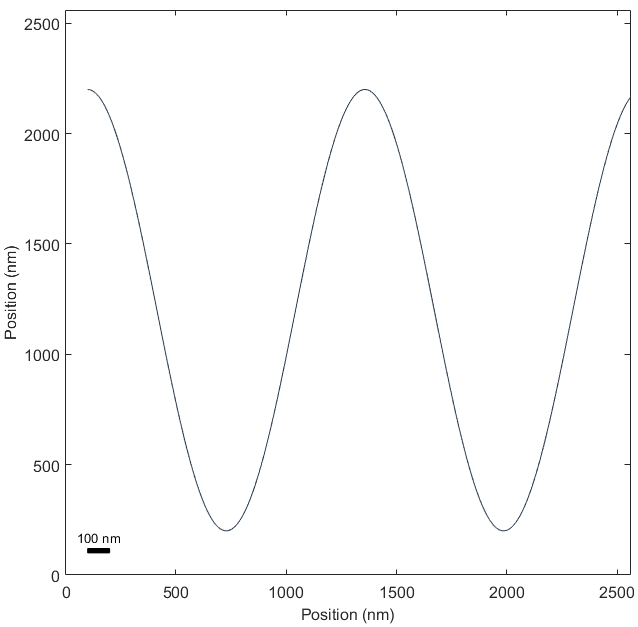
\includegraphics[width=\textwidth]{./figures/groundTruthcurve.png}
		\caption[Step1]{Ground truth shape.\newline}
		\label{fig:simStep1}
	\end{subfigure}
	\hfill
	\begin{subfigure}[b]{0.45\textwidth}
		\centering
		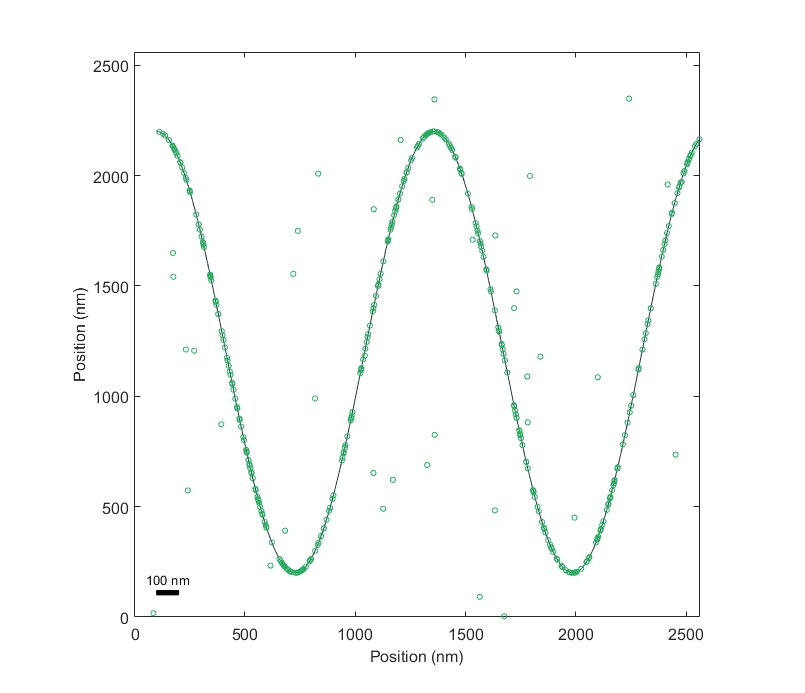
\includegraphics[width=\textwidth]{./figures/groundTruthcurveAndPoints.png}
		\caption[Step2]{Emitters (green) sparsely scattered around ground truth shape with additional points randomly distributed.}
		\label{fig:simStep2}
	\end{subfigure}
	\vskip\baselineskip
	\begin{subfigure}[b]{0.45\textwidth}
		\centering
		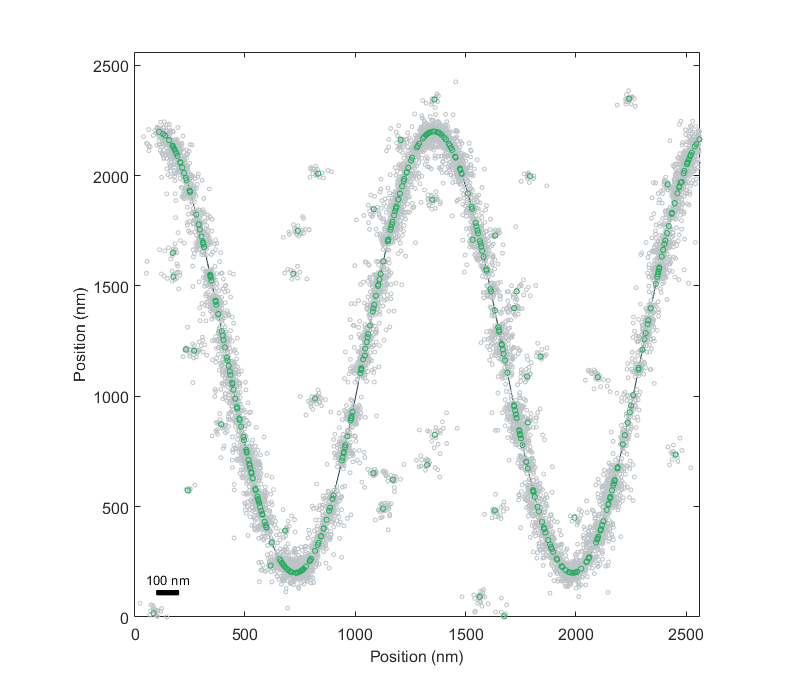
\includegraphics[width=\textwidth]{./figures/groundTruthAndSimDat.png}
		\caption[Step3]{Detection events (gray) localized around each simulated emitter.\\}
		\label{fig:simStep3}
	\end{subfigure}
	\hfill
	\begin{subfigure}[b]{0.45\textwidth}
		\centering
		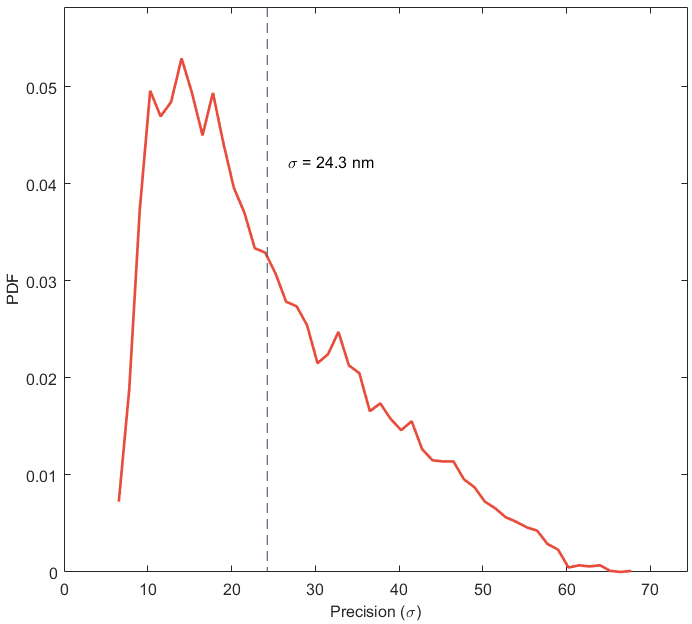
\includegraphics[width=\textwidth]{./figures/HistogramOfPrecisions.png}
		\caption[Step4]{Histogram of localization precision of simulated detection events, drawn from a distribution of experimental values, with scaling.}
		\label{fig:simStep4}
	\end{subfigure}

\caption{Steps for simulating a SMLM datset.}
\label{fig:smlmSimulation2D}
\end{figure}


These steps, represented in Figure \ref{fig:smlmSimulation2D}, proceed for both 2D and 3D simulation.  Currently 3D simulation only is supported by the repo, but 2D could be included if desired.

\subsection{3D point clouds based on test surfaces}

Input objects for 3D SMLM point cloud analysis can be provided in the STL format.  This file format represents a surface as a series of locally-flat triangles with associated nodes.  This format is commonly used for 3D printers and computer-generated objects and many programs exist for generating and manipulating these files and represented objects.  AutoDesk Fusion 360 is a freely-available CAD program I have used for generating test objects.  

Code exists in the repository to read STL files and then generate SMLM point clouds with these as the ground truth.  Function \texttt{.\textbackslash GenerateTestDataFromSTLFile.m} loads a defined STL file (using \texttt{.\textbackslash stlread.m}), scales by user-defined factor, shifts center of mass to defined position, and then generates N points randomly positioned on the loaded surface.  These then constitute the `emitter' locations.  

Function \texttt{.\textbackslash pointsToSMLMPointCloud.m} generates detection events around these emitters.  The user supplies the (x,y,z) coordinates of all emitter locations, along with the number of emitters, the mean number of detection events per emitter, and the number of detected photons and localization precision distribution to sample for this dataset.  The actual number of detection events for a given emitter is chosen as a Poisson-distributed random number with the specified mean.  The number of detected photons and localization precision distribution is pulled from an example experimental dataset (loaded using \texttt{.\textbackslash Import1File.m}).  Those simulated points whose position falls outside the specified ROI bounds are removed using \texttt{.\textbackslash enforceROIBounds.m}.  This action concludes the simulation actions, yielding a simulated 3D SMLM dataset for further processing.

\subsection{Experimentally-relevant parameters}

Within the input parameters of the simulation code, there are select variables with direct experimental corollaries. These following parameters (and \texttt{.\textbackslash MeshFitting3d.m} variable names) would be most useful in simulating various experimental outcomes:

\begin{enumerate}
	\item Emitter density (\texttt{nPoints}) - Currently defined as number of emitters per dataset.  Most relevant if converted from emitters per $\mu m^{2}$ of surface in test object.  Experimentally this pertains to specificity of label molecule, efficiency of labeling, and acquisition duration. 
	\item Detections per emitter (\texttt{nDetectsPerPoint}) - Mean number of detection events per molecule specified.  This value can be modulated experimentally by acquisition buffer chemistry, laser power, and fluorophore selection.
	\item Localization precision (implicit in \texttt{exampleDataFile}) - Values for these distributions are given \textit{via} an example data set.  It would be straightforward to model the necessary distribution as a log-Gaussian with given mean and width, or by manipulating the provided values by some scalar factor.  Experimentally the precision is a function of photons collected per detection event, which is a function of the laser power, buffer chemistry, fluorophore, and acquisition camera parameters chosen. 
	\item Off-target labeling (currently not included in 3D analysis) - The density of emitters or false positive detection events randomly distributed through the simulated ROI.  Experimentally a function of specificity of label molecule, buffer chemistry, and acquisition camera parameters chosen. 
\end{enumerate}

The inter-dependence of these parameters on the same experimental conditions makes the joint analysis of these values interesting.  For example, a given label could have high specificity, high localization precision (low values), but low emitter density and number of detections per emitter.  Another label could have lower specificity and precision, but higher emitter density and detections per emitter.  Any label could trade localization precision for additional detections per emitter (or the opposite - fewer detections per emitter but each at a higher precision) by tuning buffer chemistry and acquisition parameters.  

It is not clear which, if any, of these options is most effective to yield the highest-resolution surface as output of the next step.  One goal of this study is to determine which parameters are most essential to yield the best dataset for subsequent analysis.  

\section{Data Processing}

Data processing requires as input a 3D point cloud and a few parameters highlighted below.  The output is a mesh representation of the reconstructed surface. 

\subsection{Algorithm description}

\subsubsection{2D point cloud fitting}

The reconstruction algorithm follows the scheme outlined in \cite{lee2000curve}. Starting with an unsorted point cloud, a minimum spanning tree (\textit{via} the Delaunay triangulation) is calculated (Figure \ref{fig:fitStep1}).  This acyclic graph connects all points while minimizing the total distance traversed by all edges.  From this, the shortest path along the minimum spanning tree is calculated between the two most distant points in within this graph (Fig \ref{fig:fitStep2}). The ordered position of these points is a trajectory through the dataset roughly approximating a central path through the point cloud.  This path is smoothed and sub-sampled to more closely approximate a smooth path through the enter of the point cloud (Fig \ref{fig:fitStep3} and \ref{fig:fitStep4}).  

\begin{figure}
	\begin{subfigure}[b]{.45\textwidth}
		\centering
		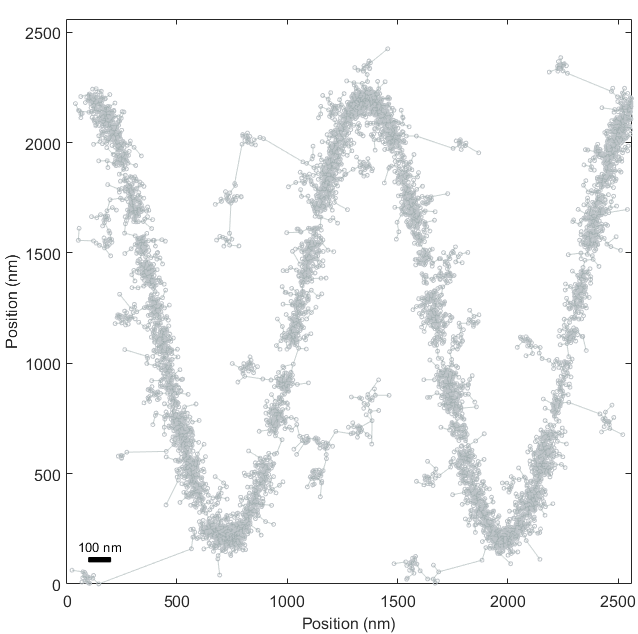
\includegraphics[width=\textwidth]{./figures/fitgraph.png}
		\caption[Step1]{Minimum span tree (lines) connecting all points in dataset (circles).}
		\label{fig:fitStep1}
	\end{subfigure}
	\hfill
	\begin{subfigure}[b]{0.45\textwidth}
		\centering
		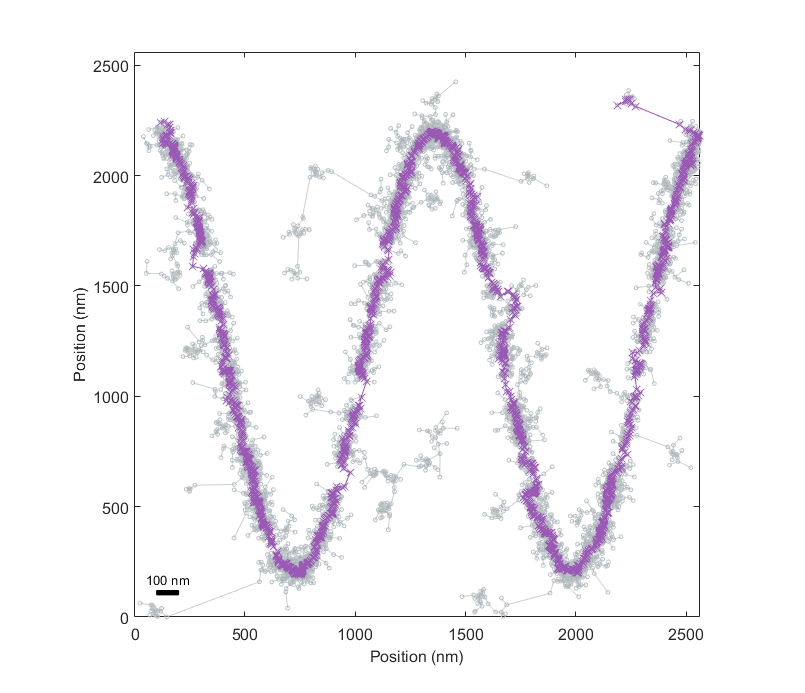
\includegraphics[width=\textwidth]{./figures/fitMinSpan.png}
		\caption[Step2]{Shortest path between most distant pair of points (purple) in the minimum spanning tree.}
		\label{fig:fitStep2}
	\end{subfigure}
	\vskip\baselineskip
	\begin{subfigure}[b]{0.45\textwidth}
		\centering
		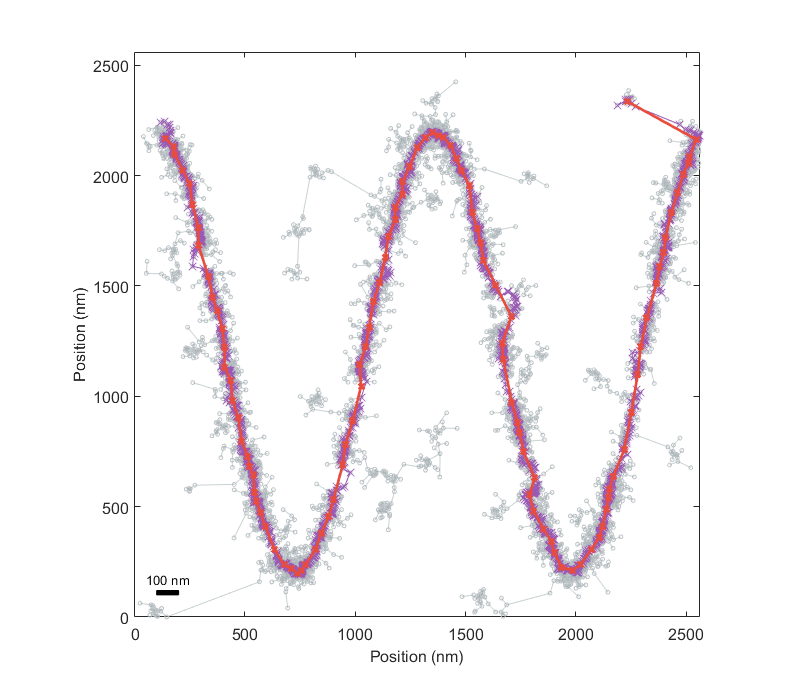
\includegraphics[width=\textwidth]{./figures/fitMinSpanAndSmooth.png}
		\caption[Step3]{Downsampled and smoothed points (red) from shortest path returned in previous step (purple).\\}
		\label{fig:fitStep3}
	\end{subfigure}
	\hfill
	\begin{subfigure}[b]{0.45\textwidth}
		\centering
		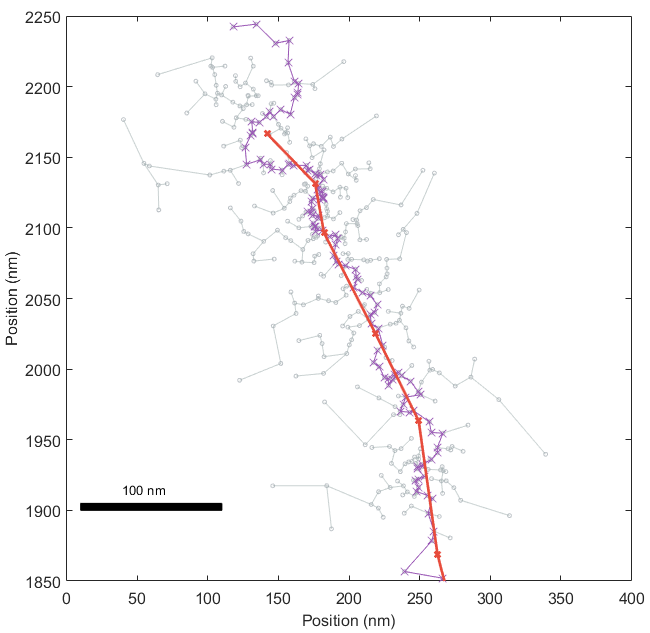
\includegraphics[width=\textwidth]{./figures/fitgraphZoom.png}
		\caption[Step4]{Zoom of initial segment in analyzed 2D dataset showing results of previous analysis steps. The initial set of shortest path points skipped prior to first fit point is apparent here.}
		\label{fig:fitStep4}
	\end{subfigure}
	
	\caption{Steps for simulating a SMLM datset.}
	\label{fig:smlmFit2D}
\end{figure}

In the implementation provided, the function \texttt{meshfigAndSmooth2d.m} calculates each 2D point cloud reconstruction using the steps above. This is called within the function \texttt{fitPointSetLoop.m}, which loops through all intersecting planes along a given axis.  

Given the complex shapes under analysis as well as presence of background signals, it is adventageous to remove overly large steps along the smoothed calculated path. Steps along this path which are significantly longer than those in the remainder of the step size distribution are suspicious and should be removed from further analysis.  These exceptionally long linkages are detected by the \texttt{rosinThreshold.m} function.  This function returns the threshold value for a `long' step in a set of smoothed paths.  The \texttt{splitByLargeDistance.m} function then separates the curve containing these distant point clouds into individual reconstruction curves.  

\begin{figure}
	\centering
	\begin{subfigure}[b]{.95\textwidth}
		\centering
		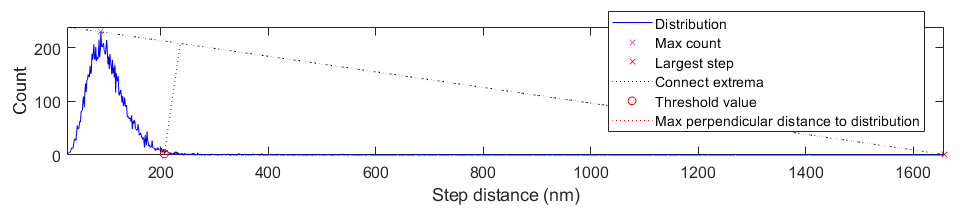
\includegraphics[width=\textwidth]{./figures/rosinThresholdDistribution.png}
		\caption[Step1]{Distribution of steps in all smoothed paths in planes of an example dataset (blue). The Rosin threshold method uses the peak and tail positions of this distribution (x markers) and finds the maximum perpendicular distance from the line connecting these points and the underlying distribution. This point (red circle) is the taken unimodal threshold value.}
		\label{fig:rosinDistribution}
	\end{subfigure}
	\begin{subfigure}[b]{.55\textwidth}
		\centering
		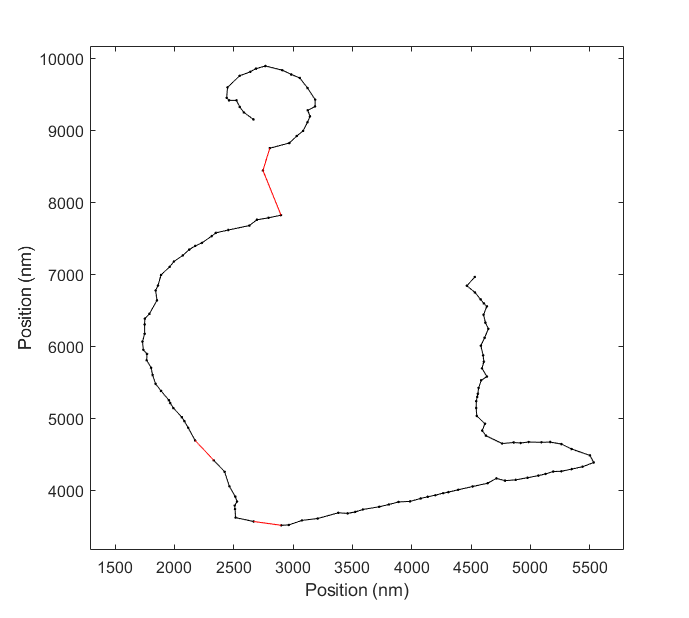
\includegraphics[width=\textwidth]{./figures/rosinThresholdPoints.png}
		\caption[Step1]{Example smoothed points plane from this dataset. Those steps in red are longer than the Rosin threshold value and should be removed. Connected points sets will be carried forward as separate reconstruction curves.}
		\label{fig:rosinPoints}
	\end{subfigure}
\end{figure}

\subsubsection{3D $\rightarrow$ 2D planes}

The above portion of the algorithm can be performed on N dimensional data, but scales poorly with a large number of points and edges.  The Prim algorithm used in MATLAB has scaling $O(E*log(N))$, where $E$ is the number of edges and $N$ the number of points in the minimum span tree.  SMLM datasets can have millions of points in the full 3D dataset, so downsampling or parcellating the calculations is prudent. 

Here this is accomplished by approximating the underlying 3D surface implied by a 3D point cloud (Figure \ref{fig:bunnyCloud}) as a set of 2D lines of intersection between the point cloud and perpendicular sampling planes (Fig \ref{fig:bunnyMeridians}).  In a single instance, a set of points close to the plane intersecting the point cloud is collapsed into a 2D plane.  This 2D point cloud is fit using the algorithm above.  The resulting reconstructed and smoothed curve, with points in 3D space representing 2D curve on intersecting plane, is returned.  This repeats at a user-specified spacing along this axis, followed by the same calculation but along the perpendicular axis.  In practice this is repeated along two more orthogonal axes, but at $\frac{\pi}{4}$ radians rotated from the first two axes.  The set of all reconstructed and smoothed curves is carried forward. 

\begin{figure}
	\centering
	\begin{subfigure}[b]{.45\textwidth}
		\centering
		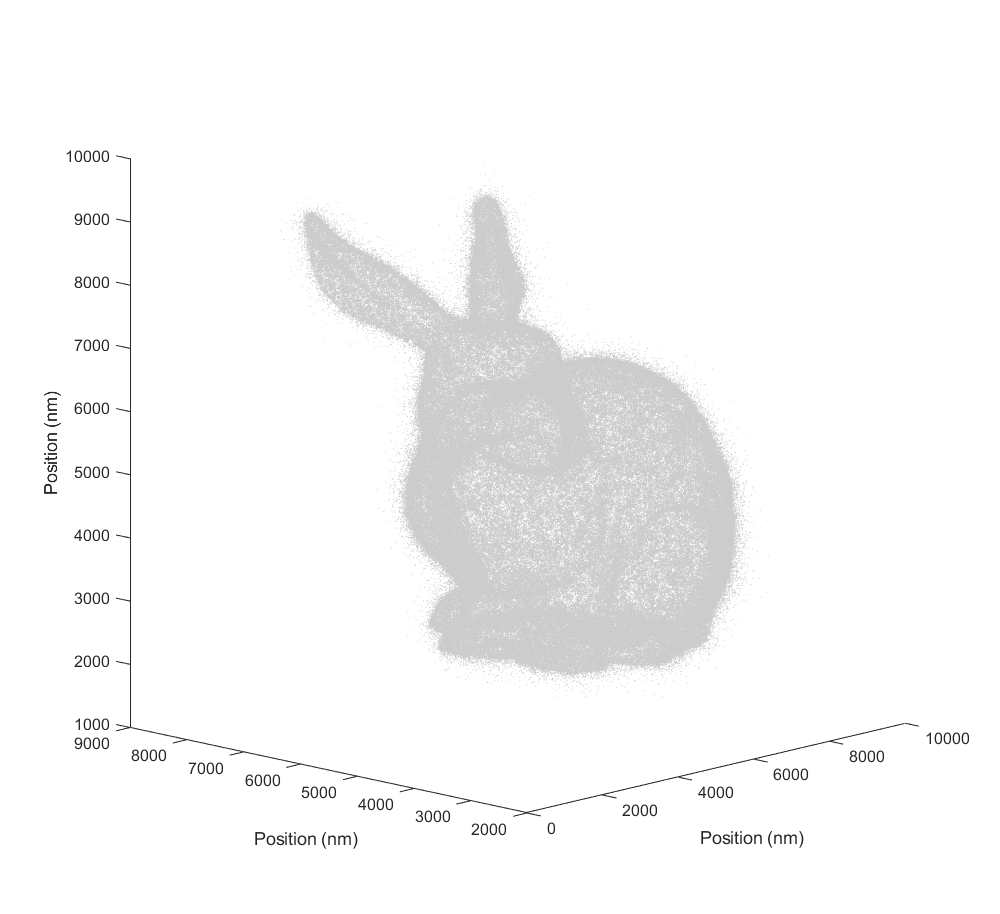
\includegraphics[width=\textwidth]{./figures/bunnyCloud.png}
		\caption[Step1]{Example 3D point cloud dataset.}
		\label{fig:bunnyCloud}
	\end{subfigure}
	\begin{subfigure}[b]{.45\textwidth}
		\centering
		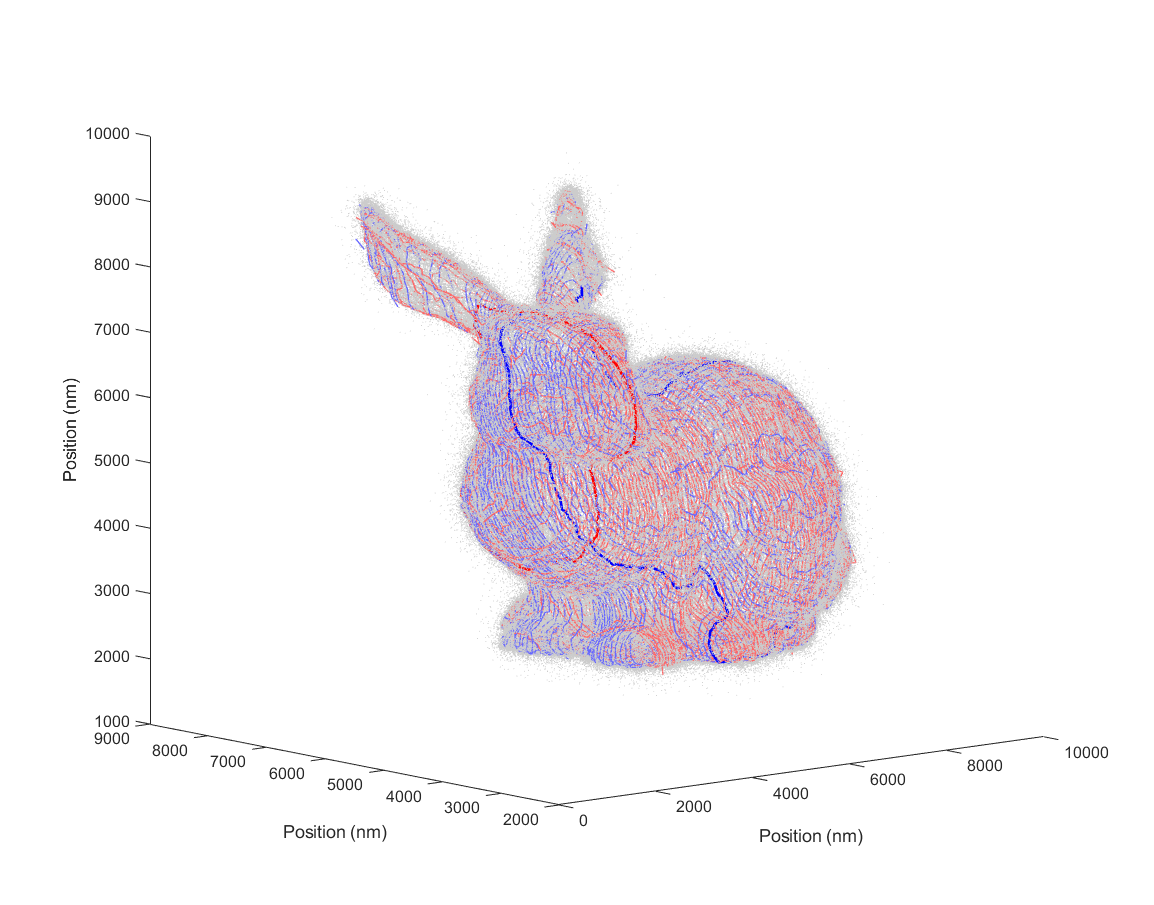
\includegraphics[width=\textwidth]{./figures/bunnyMeridians.png}
		\caption[Step2]{Reconstructed smoothed curves taken along two perpendicular planes (blur and red, respectively) intersecting the 3D point cloud dataset (gray). Single example curves from each axis highlighted.}
		\label{fig:bunnyMeridians}
	\end{subfigure}
	\vfill
	\begin{subfigure}[b]{.65\textwidth}
		\centering
		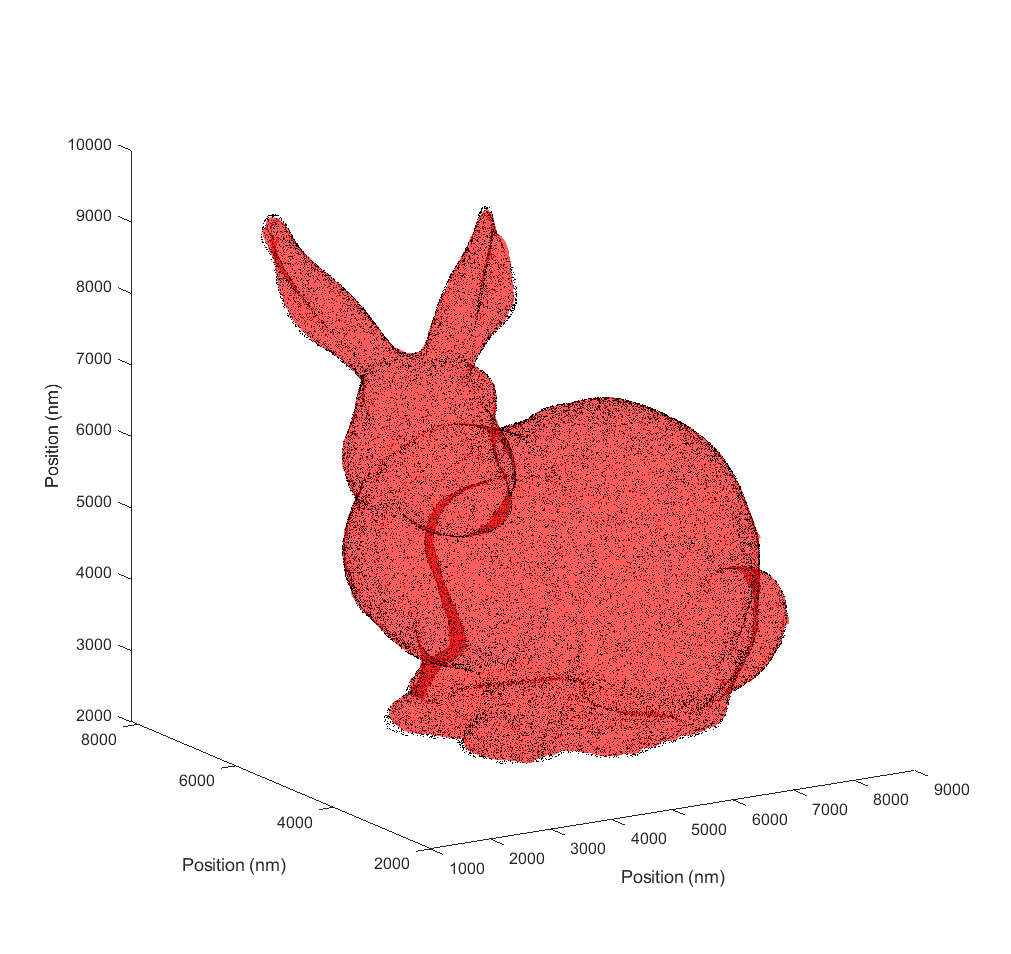
\includegraphics[width=\textwidth]{./figures/bunnyRecon+GroundTruty.png}
		\caption[Step3]{Reconstructed surface (red) with ground truth emitter points shown in black. A perfect reconstruction would yield a surface intersecting all ground truth points.}
		\label{fig:bunnyRecon}
	\end{subfigure}
\end{figure}

\subsubsection{2D fit planes $\rightarrow$ 3D volume}

From here, the surface could be passed to a surface reconstruction algorithm.  However, sampling along a third axis, orthogonal to all intersecting planes, has not occurred.  To avoid losing information due to not sampling in this direction, a further calculation is performed. 

Though originally motivated by desiring a somewhat isotropically-sampled point cloud for the surface reconstruction, it is not clear how necessary this step truly is.  It may be better to remove the Z resampling step.  This would simplify calculations while retaining the emitter density information still maintained in the intersecting plane analysis.  However, the point cloud entering the surface reconstruction step may be more noisy.  One aspect of this project should evaluate these two options to see if continuing with the resampling step here is required.  

The assembled set of all reconstructed 2D intersection lines (resampled or no) is carried forward for surface reconstruction.


\subsubsection{Surface reconstruction}

Surface reconstruction on the smoothed point cloud is accomplished using Poisson reconstruction \cite{kazhdan2006poisson} in MeshLab.  This is called through a MATLAB script invoking the MeshLab command line interface. 

The surface reconstruction algorithm returns a set of points and connectivity constituting a reconstructed surface (Fig \ref{fig:bunnyRecon}).  This reconstructed surface is the final output of the calculation and should best-approximate the ground truth object sampled through the SMLM point cloud. 

\section{Results}

Summary of accomplishments to-date:
\begin{enumerate}
	\item Implementation of simulated 3D SMLM point clouds based on STL model files.  Operates on open and closed surfaces.
	\item Algorithm for reconstruction of open or closed surfaces from noisy 3D SMLM point clouds.
	\item Implementation for reconstruction 
\end{enumerate}



\section{Continuing to completed project}

A number of improvements remain to see this reconstruction algorithm ready for tackling real and large experimental SMLM point clouds. A working list of these items are detailed below:

\subsection{Software improvements}
\begin{enumerate}
	\item \sout{Import MeshLab-provided PLY files into MATLAB as surfaces.} (Completed)
	\item Support MeshLab parameters as function arguments in \texttt{meshFitting3DFcn.m}.
	\item Potentially implement new smoothing method based on Lee publication for 2D reconstructed curves.
	\item Software implementation of the pointillist Fourier shell correlation algorithm. 
\end{enumerate}

\subsection{Algorithm parameterization}
\begin{enumerate}
	\item Compare reconstruction performance between Z-resampled point cloud (current implementation) and direct operation of Poisson reconstruction on smoothed 2D reconstructed curve points.
\end{enumerate}

\subsection{Quantifying performance}
There is a great need for a means to quantify the performance of the reconstruction algorithm in terms of resolution of feature which can be resolved in the output surface. This could be evaluated with increasing levels of complexity (and usefulness).  Any of these analyses should allow the quantification of the achievable resolution under a given set of point cloud and algorithm parameters.  This should be used to benchmark the optimum algorithm parameters for reconstruction and to inform the cut-off for valid biological interpretation from a given experimental dataset. 

\begin{enumerate}
	\item \textbf{RMS error relative to ground truth} - When a known input structure is known, the output of the reconstruction can be referenced to this ground truth. This provides a straightforward means to assess how close the reconstruction can match the input structure.  
	
	A challenge of comparing two surfaces is finding elements on both surfaces to align for comparison.  A possible implementation would be to take the distance from the ground truth emitter positions (returned as the \texttt{groundTruth} output from \texttt{meshFitting3DFcn}) to the nearest surface element on the returned reconstruction.  If the size of the facets of the reconstructed surface is small, then the distance from a ground truth point to the nearest vertex of the reconstruction surface can be a reasonable approximation of the ground truth point to reconstruction facet distance.  This point-to-point distance is straightforward to calculate with a k nearest neighbor algorithm. 
		
	Unfortunately this approach does not directly return any information regarding the feature size of the surface relative to the error observed. It is expected that areas of high spatial frequency in the underlying structure would have higher error in the reconstruction relative to `flatter' regions. 
	
	\begin{figure}
		\centering
		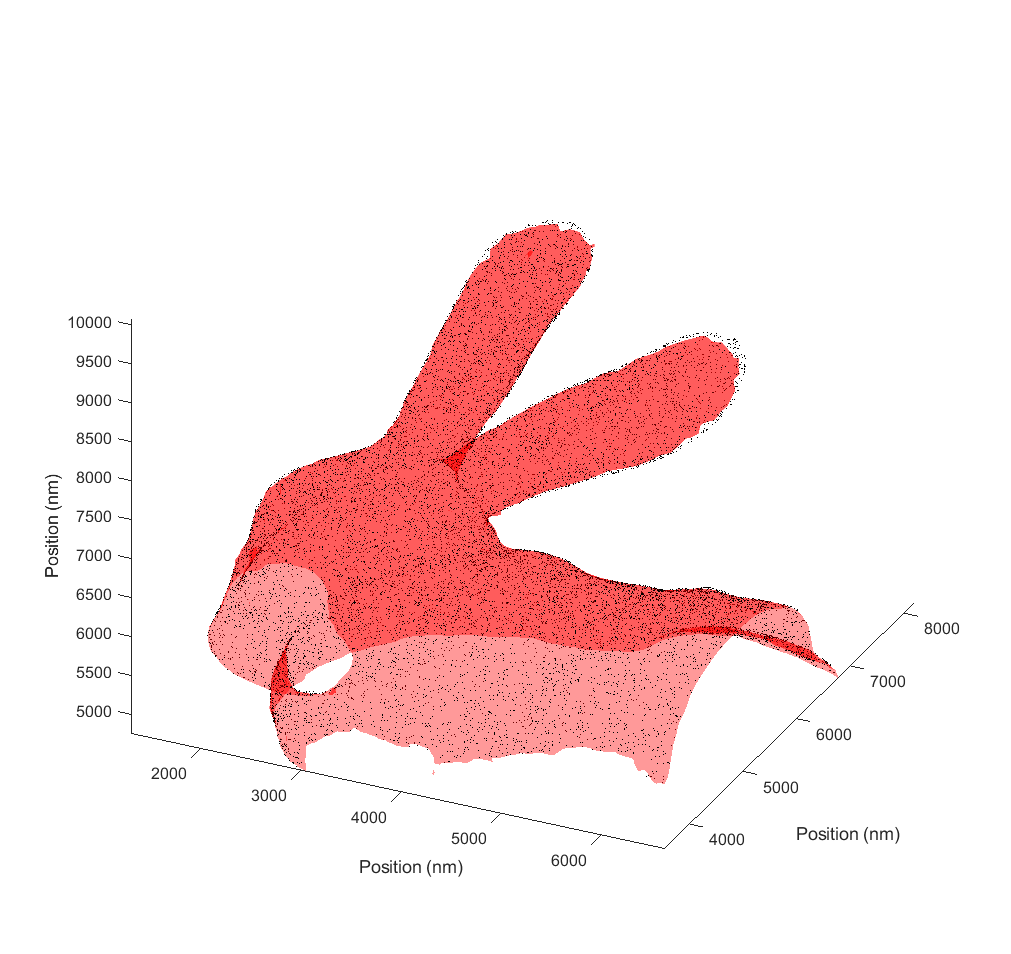
\includegraphics[width=0.5\textwidth]{./figures/bunnyReconEars.png}
		\caption[Step3]{Zoom of reconstructed surface and ground truth points appearing in \ref{fig:bunnyRecon}.  Note that at the sharp point of the ears, or the area of highest extent and spatial frequency, the reconstructed surface does not match the extent of the ground truth surface.}
		\label{fig:bunnyReconModulation}
	\end{figure}
	
	\item \textbf{Modulation depth in a periodic surface} - Given the nature of the 2D and 3D reconstruction methods, it is anticipated that features below the reconstruction resolution will be truncated or `cut off'.  With a simulated surface the spatial frequency of the underlying features can be easily parameterized.  With this it is possible to design a series of tests in which the spatial frequency is increased while evaluating the surface reconstruction error at each point.  
	
	\begin{figure}
		\centering
		\begin{subfigure}[b]{.3\textwidth}
			\centering
			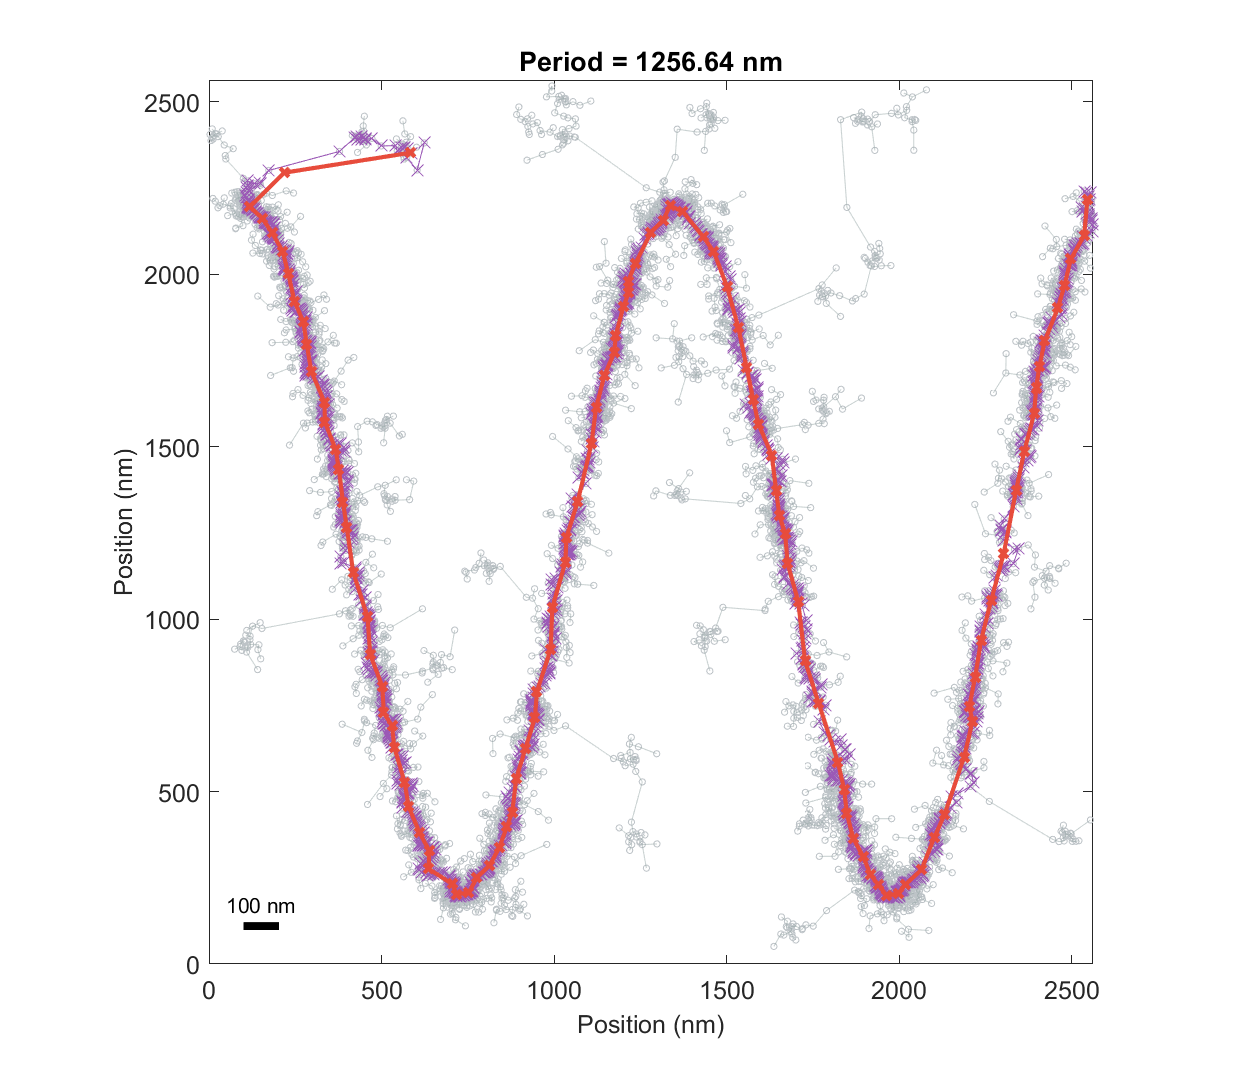
\includegraphics[width=\textwidth]{./figures/FitPoints2d_pts-400_period-1256.png}
			\caption[Step1]{}
			\label{fig:modDepth400_fDiv10}
		\end{subfigure}
		\begin{subfigure}[b]{.3\textwidth}
			\centering
			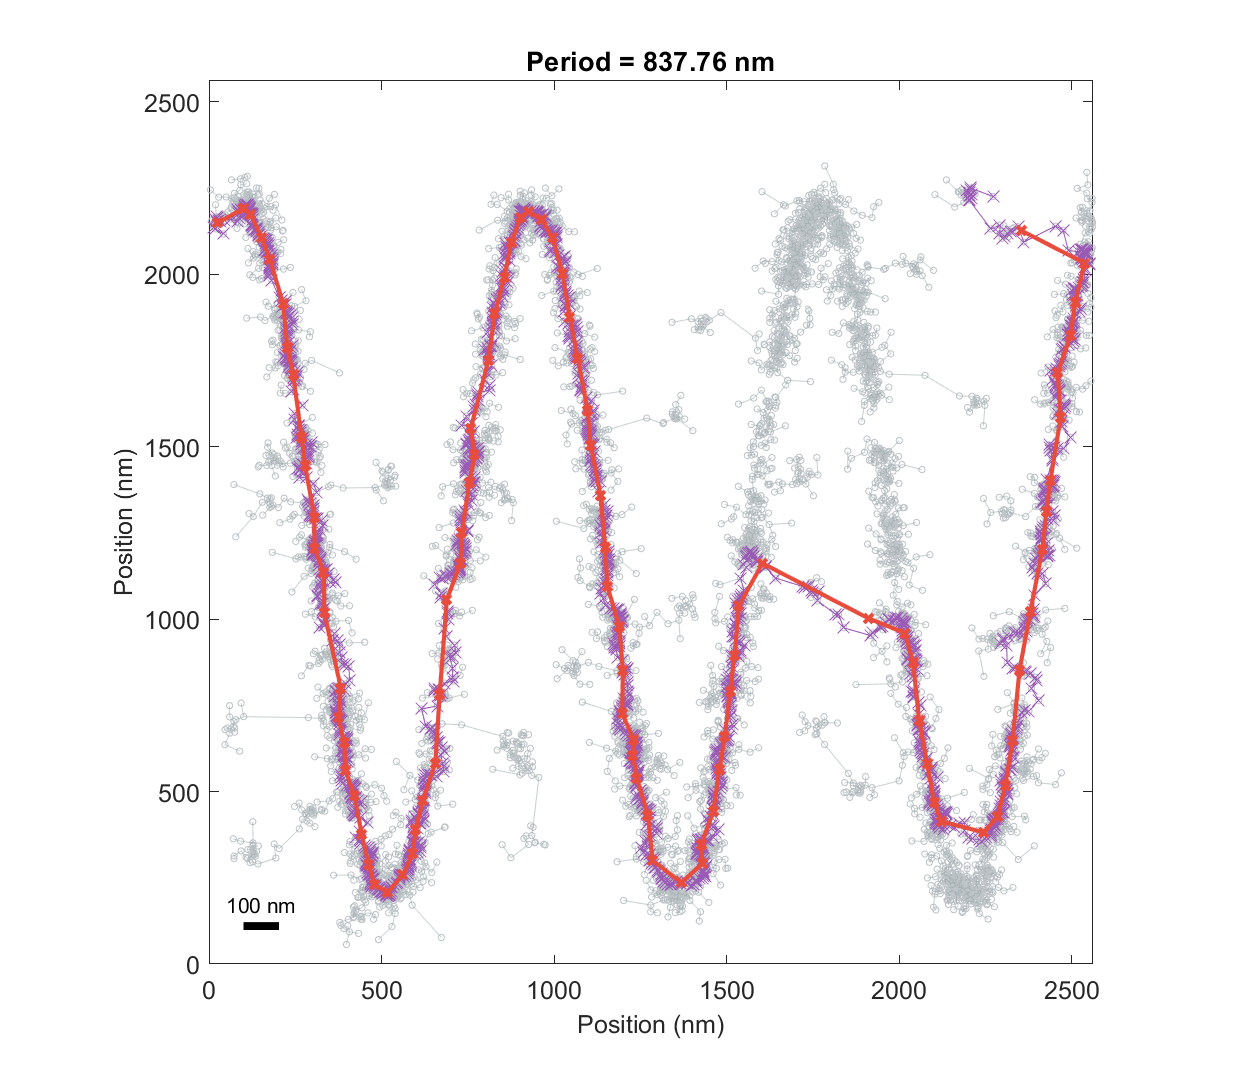
\includegraphics[width=\textwidth]{./figures/FitPoints2d_pts-400_period-837.png}
			\caption[Step2]{}
			\label{fig:modDepth400_fDiv15}
		\end{subfigure}
		\begin{subfigure}[b]{.3\textwidth}
			\centering
			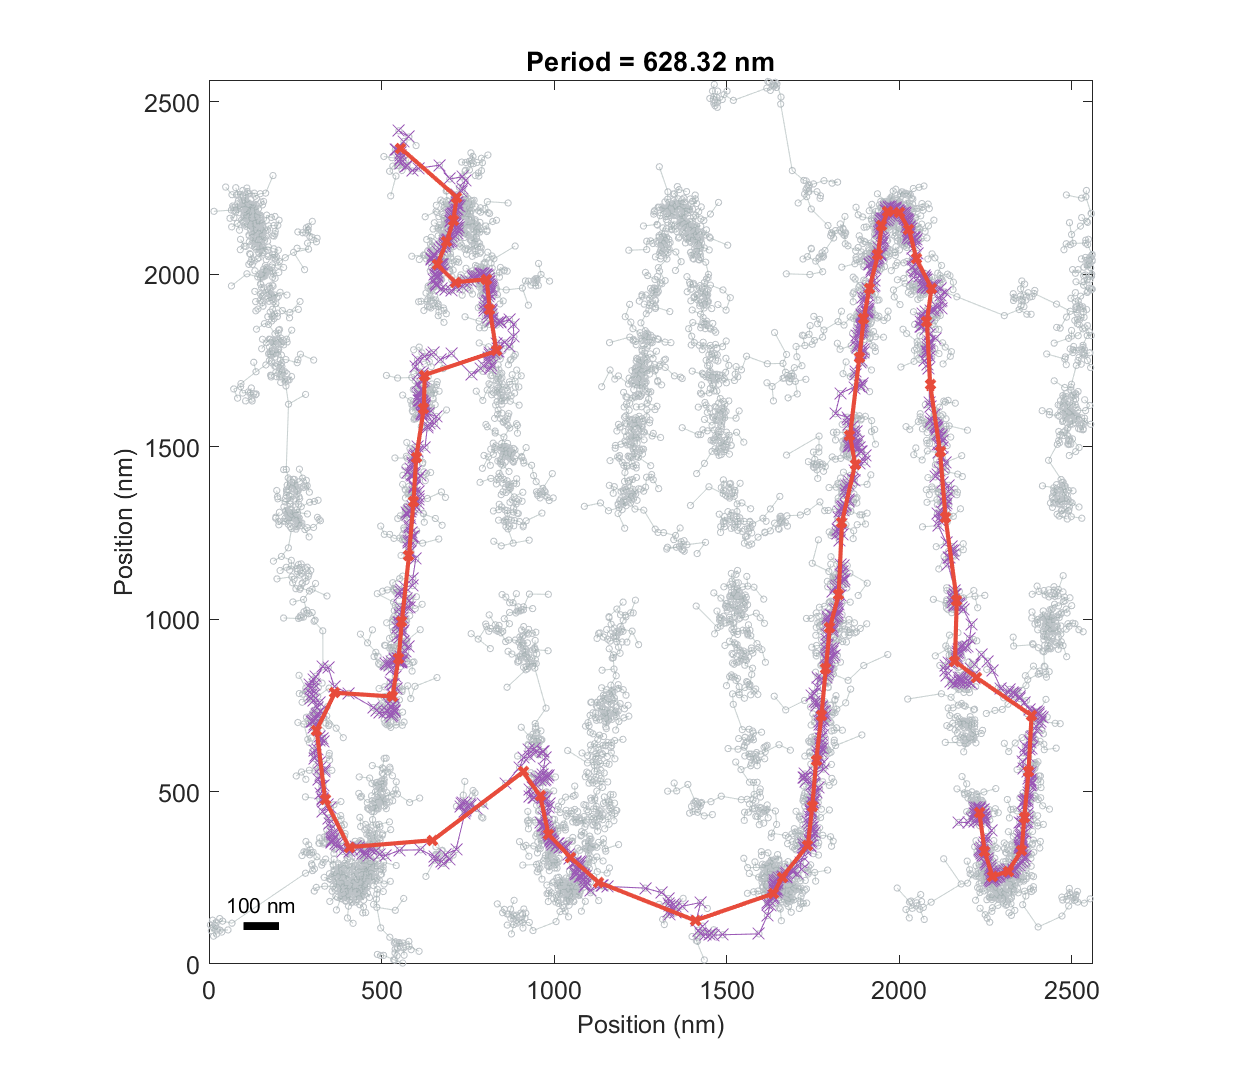
\includegraphics[width=\textwidth]{./figures/FitPoints2d_pts-400_period-628.png}
			\caption[Step2]{}
			\label{fig:modDEpth400_fDiv20}
		\end{subfigure}
	
	\vskip\baselineskip
	
			\begin{subfigure}[b]{.3\textwidth}
		\centering
		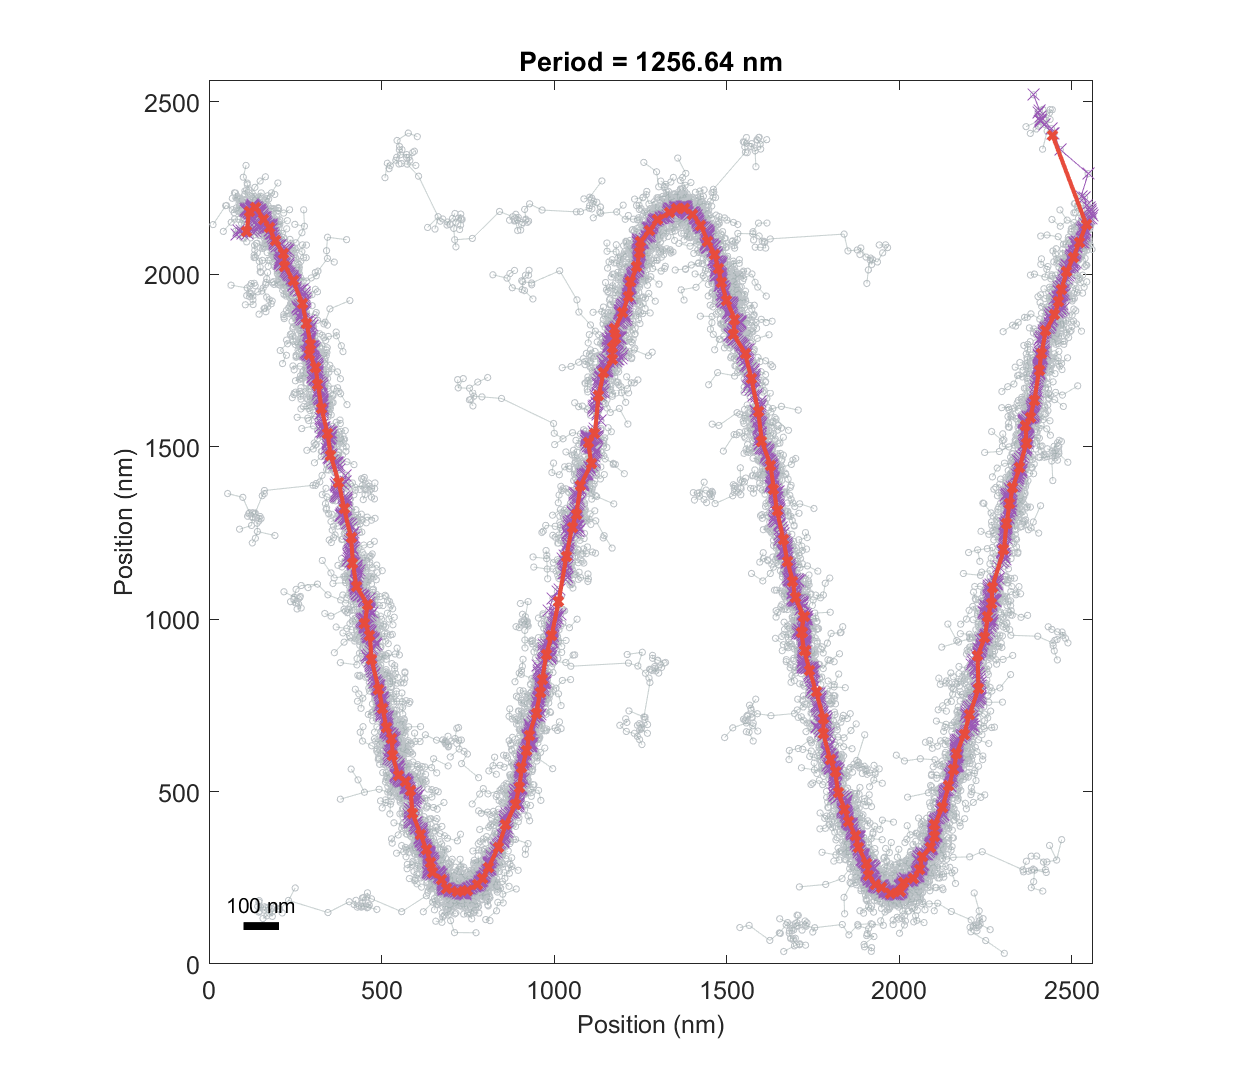
\includegraphics[width=\textwidth]{./figures/FitPoints2d_pts-800_period-1256.png}
		\caption[Step1]{}
		\label{fig:modDepth800_fDiv10}
	\end{subfigure}
	\begin{subfigure}[b]{.3\textwidth}
		\centering
		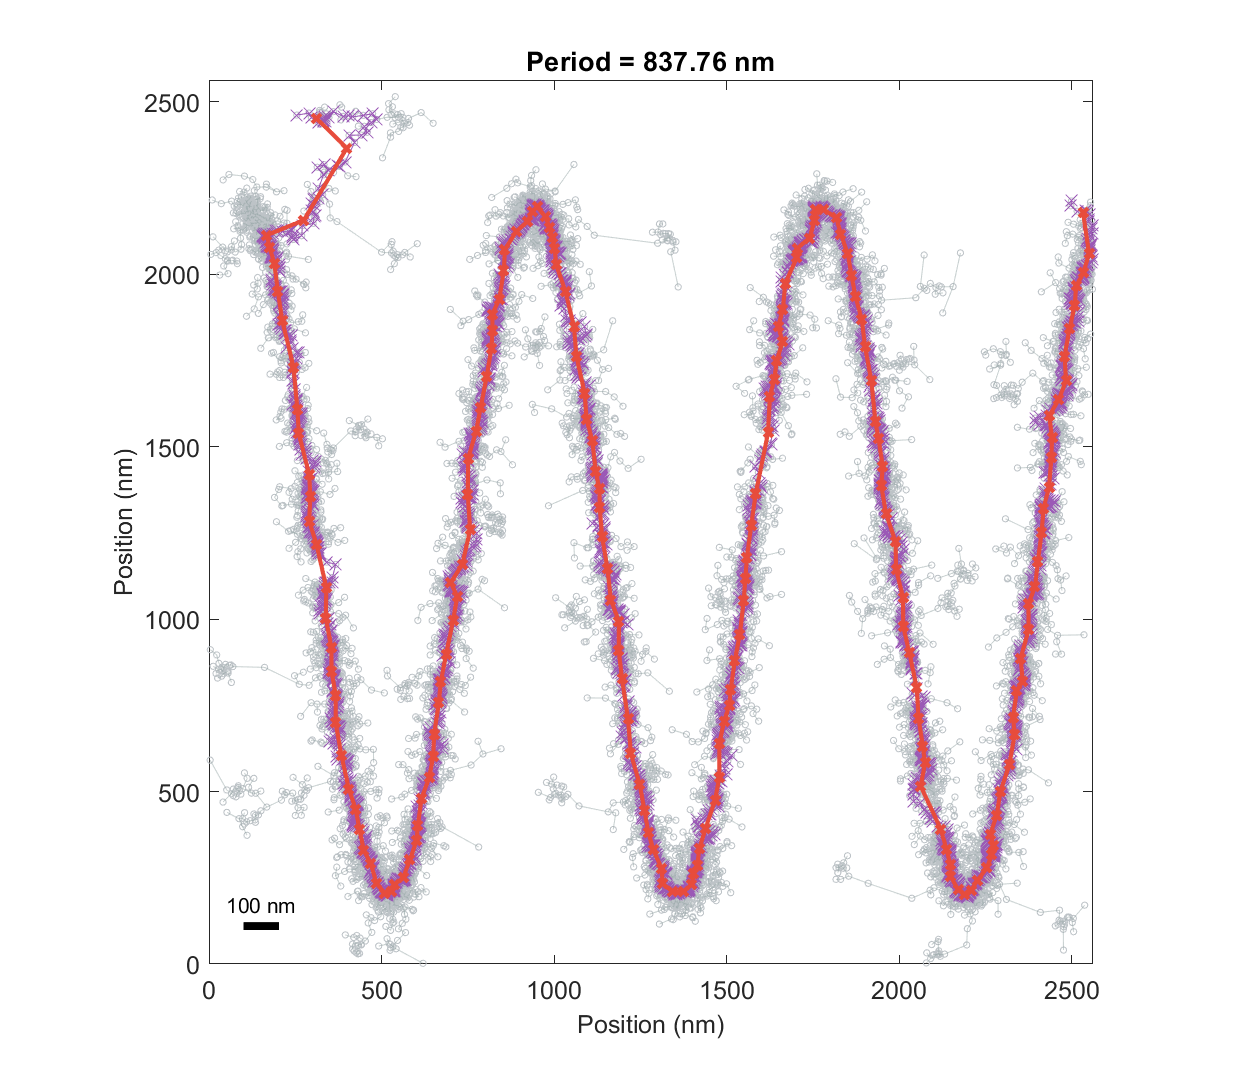
\includegraphics[width=\textwidth]{./figures/FitPoints2d_pts-800_period-837.png}
		\caption[Step2]{}
		\label{fig:modDepth800_fDiv15}
	\end{subfigure}
	\begin{subfigure}[b]{.3\textwidth}
		\centering
		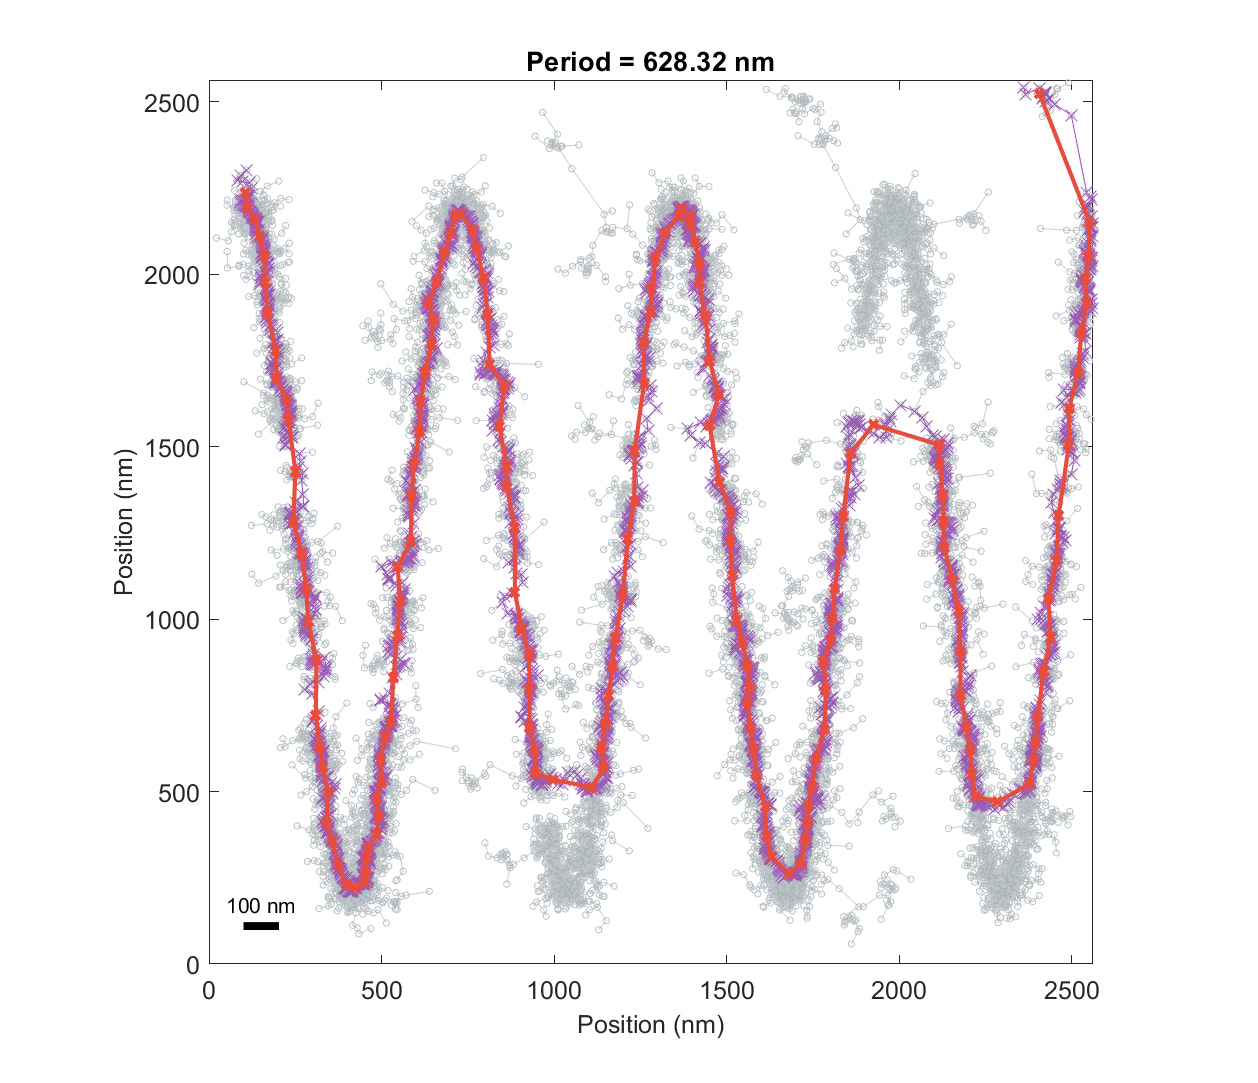
\includegraphics[width=\textwidth]{./figures/FitPoints2d_pts-800_period-628.png}
		\caption[Step2]{}
		\label{fig:modDEpth800_fDiv20}
	\end{subfigure}

	\vskip\baselineskip
	
	\begin{subfigure}[b]{.3\textwidth}
		\centering
		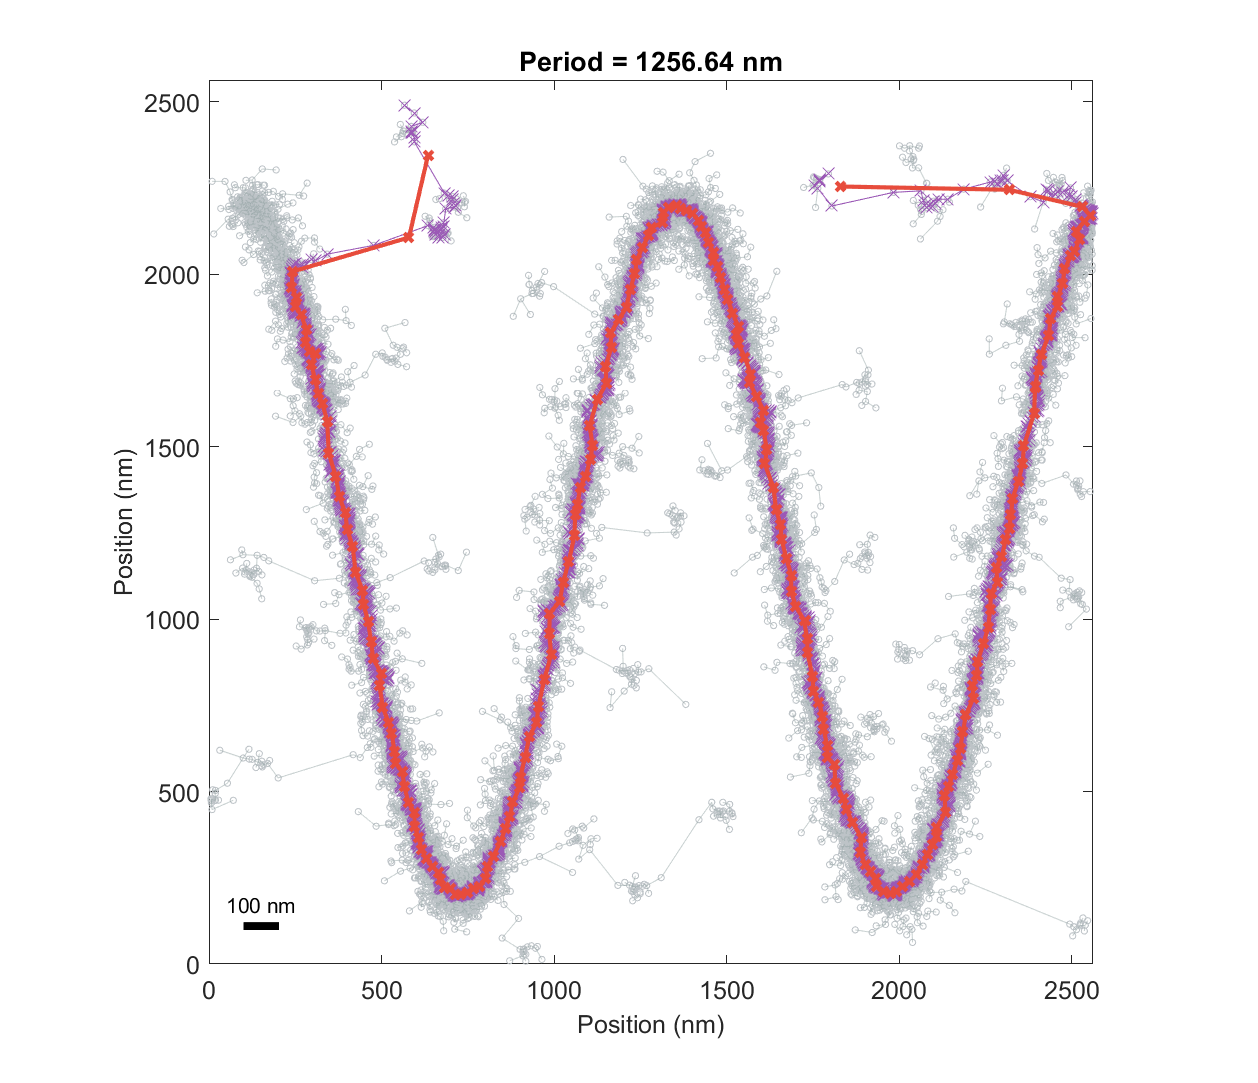
\includegraphics[width=\textwidth]{./figures/FitPoints2d_pts-1200_period-1256.png}
		\caption[Step1]{}
		\label{fig:modDepth1200_fDiv10}
	\end{subfigure}
	\begin{subfigure}[b]{.3\textwidth}
		\centering
		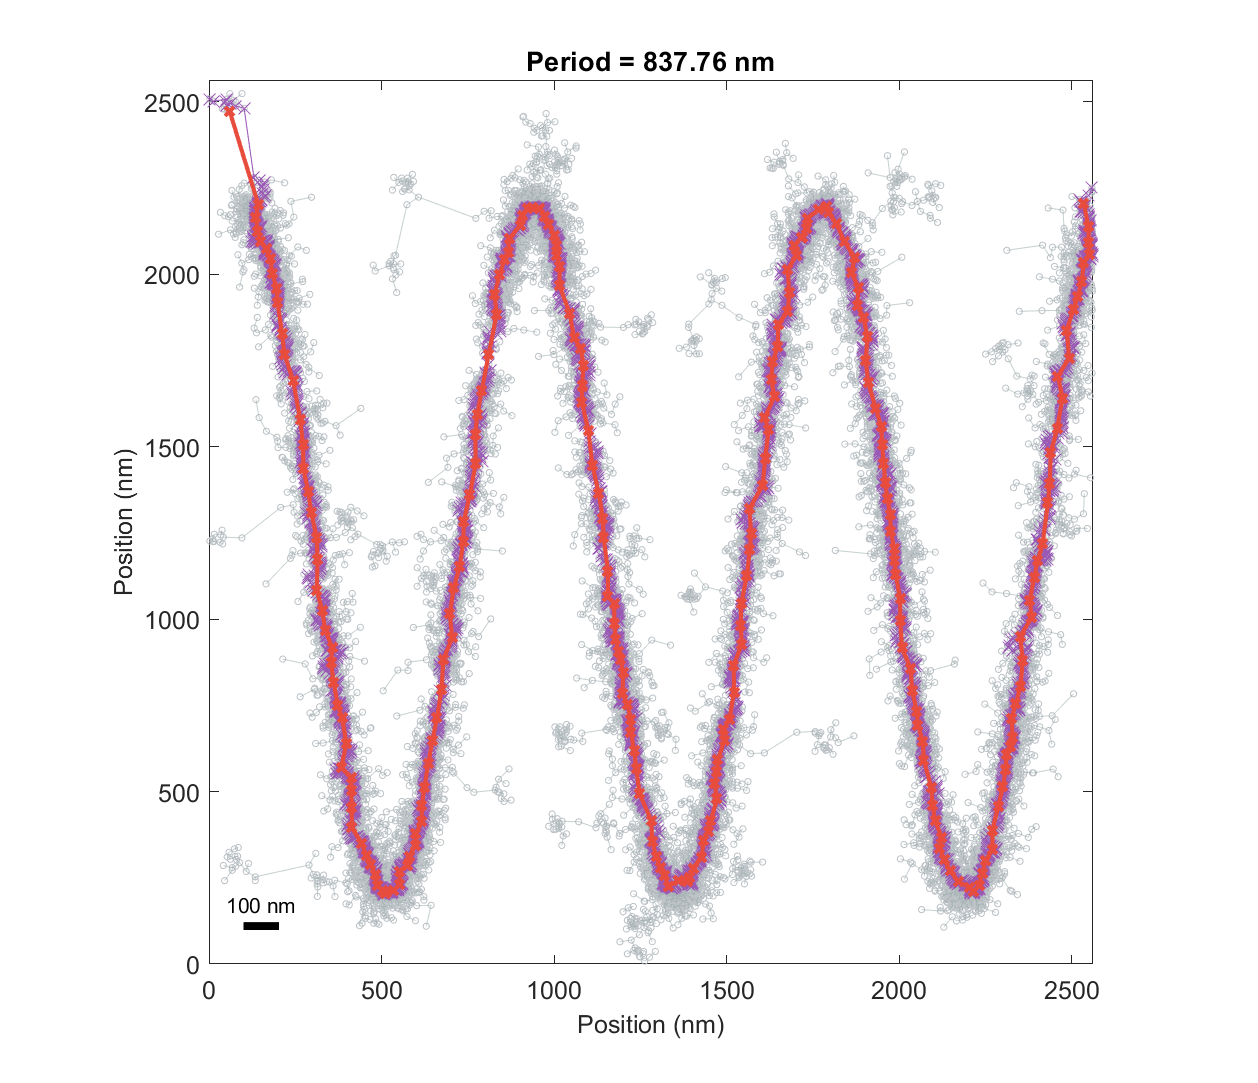
\includegraphics[width=\textwidth]{./figures/FitPoints2d_pts-1200_period-837.png}
		\caption[Step2]{}
		\label{fig:modDepth1200_fDiv15}
	\end{subfigure}
	\begin{subfigure}[b]{.3\textwidth}
		\centering
		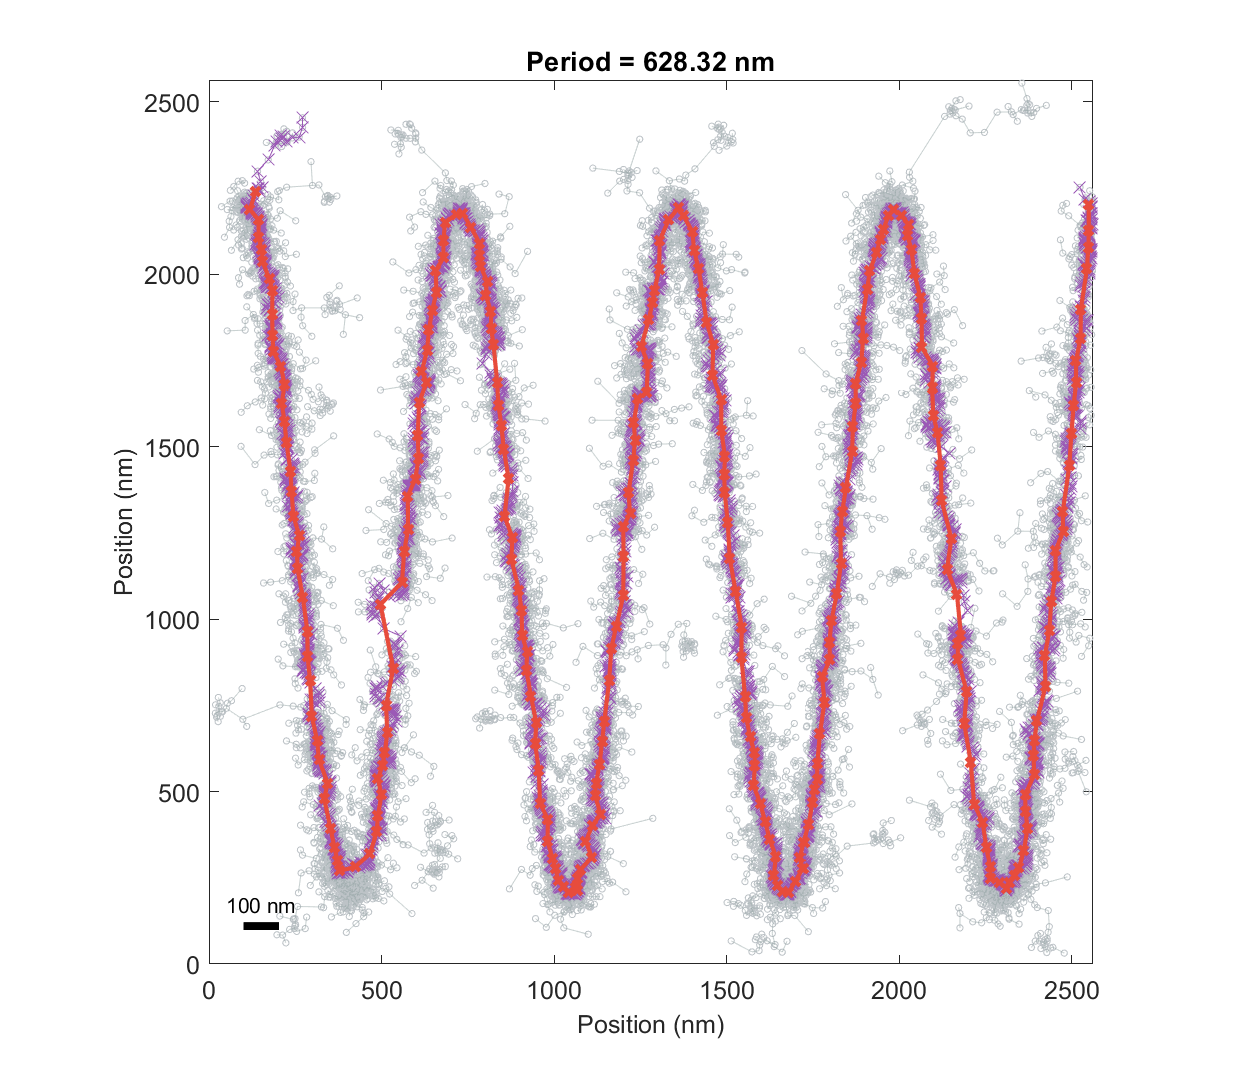
\includegraphics[width=\textwidth]{./figures/FitPoints2d_pts-1200_period-628.png}
		\caption[Step2]{}
		\label{fig:modDEpth1200_fDiv20}
	\end{subfigure}	

\caption{Fidelity of reconstruction is affected by spatial frequency of input structure relative to number of sampled points. A cosine function of indicated spatial frequency defines ground truth structure and fit using described algorithm for single-plane reconstruction (see Figures \ref{fig:smlmSimulation2D} and \ref{fig:smlmFit2D}). \ref{fig:modDepth400_fDiv10} - \ref{fig:modDEpth400_fDiv20} simulated with 400 points around this ground truth, \ref{fig:modDepth800_fDiv10} - \ref{fig:modDEpth800_fDiv20} with 800 points, and \ref{fig:modDepth1200_fDiv10} - \ref{fig:modDEpth1200_fDiv20} with 1200 points.  The reconstructed curve (red) shows clipping at the extrema when sampling is insufficient for the spatial frequency in question.  A similar response would be expected for a number of experimental parameters. } \end{figure}
	
	
	One approach is to generate a series of surfaces following a sine or square wave pattern with a given spatial frequency.  Measuring the reconstruction error as a function of a simulation or algorithm parameter would yield a response function for that combination of parameters.  Taking each parameter in turn, along with the spatial frequency of the simulated surface, would yield a multidimensional response function for the algorithm.  These results can be used as a lookup table against which experimental data and interpretation can be referenced.
	
	\item \textbf{Fourier ring correlation} - The Fourier ring correlation algorithm (\cite{nieuwenhuizen2013measuring}, \cite{salas2017angular}) provides a means to directly estimate the achievable resolution from a given dataset.  These give a direct readout of response as a function of spatial frequency from a single experimental reconstruction without any ground truth reference. This form will be most useful for quantifying the interpretation level possible for an experimental dataset directly.  Such a readout would efficiently parameterize results from simulations as well. 

	Two-dimensional implementations of the Fourier ring correlation have been long used for quantifying cryo-EM and crystallography reconstructions. Three-dimensional forms (the Fourier shell correlation) is a straightforward extension of the two-dimensional form.  Image-based forms are most common and not necessarily the optimal form for pointillist datasets.
	
	A recent preprint describes a pointillist form of the Fourier ring correlation algorithm (\cite{8759279}).  This would be the most direct route to quantifying resolution in both simulated and experimental datasets.  At the moment a freely-available software implementation is not in hand.  If not possible to recapitulate this analysis from the described methods then it may be possible to discuss with the preprint authors regarding their software.
	
\end{enumerate}

\bibliography{smlm3dmeshfitting}
	
\end{document}